%++++++++++++++++++++++++++++++++++++++++
% Don't modify this section unless you know what you're doing!
\documentclass[letterpaper,11pt]{article}
\usepackage{tabularx} % extra features for tabular environment
\usepackage{amsmath}  % improve math presentation
\usepackage{graphicx} % takes care of graphic including machinery
\usepackage[margin=0.8in,letterpaper]{geometry} % decreases margins
\usepackage{cite} % takes care of citations
\usepackage[final]{hyperref} % adds hyper links inside the generated pdf file
\usepackage{subfigure}
\usepackage[font=small,labelfont=bf]{caption}
\usepackage{layout}
\hypersetup{
	colorlinks=true,       % false: boxed links; true: colored links
	linkcolor=blue,        % color of internal links
	citecolor=blue,        % color of links to bibliography
	filecolor=magenta,     % color of file links
	urlcolor=blue         
}
% \addtolength{\voffset}{-30pt}
%++++++++++++++++++++++++++++++++++++++++

\begin{document}

\title{CSE291 Course Project Part I Report}
\author{Wenshuo Zang,  Zhaofang Qian}
\date{\today}
\maketitle
\setlength{\parindent}{20pt}
\vspace{-2em}
{ \scriptsize {The results link: \url{https://drive.google.com/drive/folders/12-EF52mNqfiQgLc0iGvZ2sLgkiIA-N1r?usp=sharing}}}

\section{LiftCube}
In this task, the agent of a seven-joint manipulator is trained by Proximal Policy Optimization(PPO)\cite{ppo}. We started with the 
parameters given by the tutorials of Maniskill2, and the results are shown in the first row of table~\ref{table:ppo}.
The initial training took a little bit long, around twenty minutes. To increase the speed, the number of environments(env)
is set to eight, since they contributes to the same Q-network. But the result doesn't not manifest any improvement.
The reason is that the number of steps for each env is equal to total rollout steps divided by number of envs.
Each env seemed to be lack of steps to collect enough info for time difference computation. Either increasing the 
total rollout steps or changing back. To verify the rest of parameters, we decided to only have two environments.
Then we tried to increase the batch size, finding that the larger batch size, the higher the slope of mean reward pre
epsoide is, indicating that this reward curve would increase faster to reach the goal. Just as shown in fig~\ref{fig:ppo2}(b),
the purple curve is 512 batch size and others are 128 and 256 instead. Hence the 512 batch size was selected.

At this time, we didn't realize the most important parameter, reward or discounted factor, should be tuned first, as
instructor mentioned during the class. We only can change $\gamma$ to impact the rewards. The large factors weighted
more future returns, while the small factors focused on more "myoptic" results. We increased $\gamma$ to $0.95$,
and got a similar result, which indicates that the large discounted factor failed in converging the neural networks.
After a few experiments, when the factor is 0.7, PPO can completely handle the task. In this case, the training loss
remained at a low level in blue curves of Fig~\ref{fig:ppo2}(d). This Python library implements
a GAE+PPO method. We wanna to see how the GAE factor $\lambda$ impacts results. Due to the limitation of samples, 
the advantage function has to balance the variance and bias. The smaller $\lambda$ manifests smaller variance but larger
bias. We played with different $\lambda$ values from 0.95 to 0.999 and found the best is the default value. All results are 
presented in table.\ref{table:ppo} for the convenience of comparsion.

\begin{table}[h!]
    \centering
    \begin{tabular}{||c c c c c c c c c||} \hline
      Test No. & $\gamma$ & batch\textunderscore size & env\textunderscore num & samples & steps & epochs & $\lambda$ & Success\\ [0.5ex] 
      \hline\hline
      1 & 0.85 & 256 & 2 & 400k & 4096& 15 & 0.95 & 0.5 \\ 
      2 & 0.85 & 256 & 8 & 400k & 4096& 15 & 0.95 & 0.3 \\
      3 & 0.85 & 512 & 2 & 400k & 4096& 15 & 0.95 & 0.4 \\
      4 & 0.95 & 512 & 2 & 400k & 4096& 15 & 0.95 & 0.5 \\
      5 & 0.70 & 512 & 2 & 400k & 4096& 15 & 0.95 & 1.0 \\
      6 & 0.70 & 512 & 2 & 400k & 4096& 15 & 0.97 & 0.9 \\ 
      [1ex] \hline
    \end{tabular}
  \caption{Parameters of PPO in LiftCube-v1}
  \label{table:ppo}
\end{table}

\begin{figure}
  \centering
  \subfigure[]{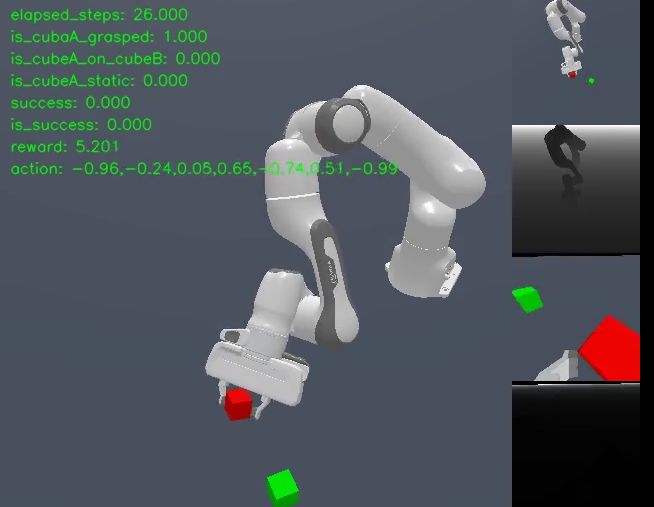
\includegraphics[width=0.21\textwidth]{figs/ppo1.png}} 
  \subfigure[]{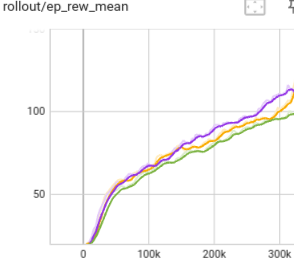
\includegraphics[width=0.21\textwidth]{figs/ppo2.png}} 
  \subfigure[]{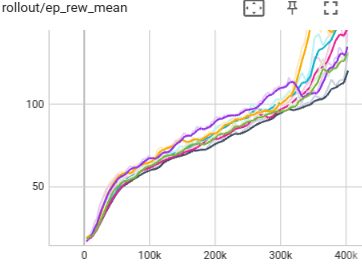
\includegraphics[width=0.24\textwidth]{figs/ppo3.png}}
  \subfigure[]{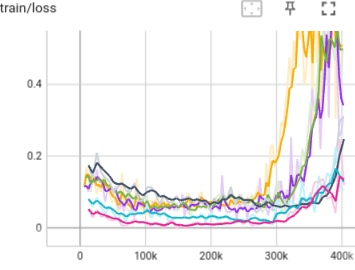
\includegraphics[width=0.24\textwidth]{figs/ppo4.png}}
  \caption{(a)PPO StackCube in local optima (b) PPO avg\textunderscore reward various batch sizes 
  (c) PPO avg\textunderscore reward (d) PPO train loss}
  \label{fig:ppo2}
\end{figure}


\section{StackCube}
This task consists of three movements, which are lifting the cube, moving to the top of the other, and dropping the cube.
After finishing each, the agent would get rewards, but easily stuck in local optima by using PPO. We frequently 
observed in videos that the manipulator stayed static all the time immediately one of the movements was done. Since the exploration 
of PPO algorithm relied on action samples correspongding to the most recent stochastic polices, both the initial conditions
and the training processes determined the sampled actions' randomness. Then, the policy network gradually lost the randomness and 
instead exploited the rewards as much as it could. Therefore, another algorithm, Soft Actor-Critic(SAC)\cite{sac}, was applied to 
prevent the agent from trapped into local optima. 

% batch size, learning rate, ent_coef, learnig starts, gamma
\begin{figure}[ht] 
  \centering
  \subfigure[]{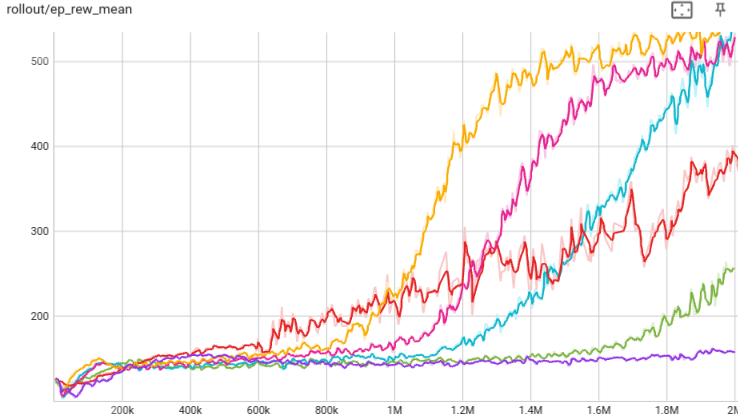
\includegraphics[width=0.49\textwidth]{figs/sac1.png}} 
  \subfigure[]{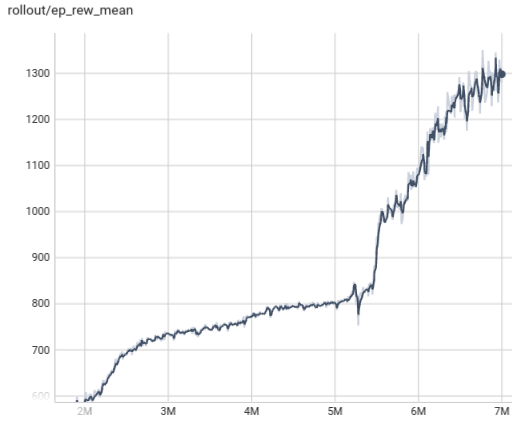
\includegraphics[width=0.33\textwidth]{figs/sac2.png}} 
  \captionsetup{justification=centering}
  \caption{(a)SAC Average rewards per eposide (Test 1-6) \\
  (b)SAC Average rewards per eposide of the successful tuning (Test 7)}
    \label{fig:sac1}
\end{figure}

SAC is a stochastic off-policy method incorporating entropy regularization and clipped double-Q trick.
First, we tried the default parameters provided by stable\textunderscore baseline3 and got a bad result, 
as shown in the first row of table ~\ref{table:sac}. 
The most important two key parameters are reward(or discounted factor $\gamma$) and update interval (the ratio to 
env\textunderscore steps) and every tuning should start with these two. After increasing $\gamma$ to 0.95, 
the model doesn't converge at all and the rewards remained relatively stable at a low value, as the green curve shown in 
figure~\ref{fig:sac1}(a). Then, we tried a smaller discounted factor, 0.85 and the eposide mean reward curve 
increased a little bit. After several trials, the best $\gamma$ is 0.9, and the comparsion are presented in 
table ~\ref{table:sac}. Next, we tried different update interval correspongding to the update\textunderscore freq in table.
This parameter controls updating the model every "train\textunderscore freq" steps. 
The suitable update interval is 1 after some experiments. Because when increasing the frequency to 2, the 
rewards didn't not grow gradually, just like the cyan color one in figure~\ref{fig:sac1}(a). So far, we have
tuned the dominating hyperparameters. Subsequently, we move to some special parameters of SAC.

The value function of SAC is given by 
\begin{equation}
  V^{\pi}(s) = E_{\tau \sim \pi}(Q(s_t,a_t) + \alpha H(\pi( \cdot | s_t))) \nonumber
\end{equation}
If we write the above in the supervised learning convention, it is equivalent to 
\begin{equation}
  \mathcal{L}_{actor} = \lambda_1 \mathcal{L}_{reward} + \lambda_2 \mathcal{L}_{entropy} \nonumber
\end{equation}
, where $\mathcal{L}_{reward}$ allows actor's policy gains larger and larger returns from critic, and 
$\mathcal{L}_{entropy}$ increases the entropy of the policy of actor. As we know, the entropy can helps the exploration
so we have to balance it with exploitation. Thus, reward scaling is introduced to meet the requirements. The parameter,
entropy\textunderscore coeff is equal to the inverse of reward scaling. When increasing it, the total returns grows faster
but suffered from stability issues. From the red curve corresponding to test 3 in figure~\ref{fig:sac1}(a), the reward
is shaking all the time, indicating too much random exploration. Therefore, we should tune it down. The desired value
is 0.08. In this case, the reward incremental is very stable.

\begin{table}[h!]
  \centering
  \begin{tabular}{||c c c c c c c ||} \hline
    Test No. & $\gamma$ & batch\textunderscore size & entropy\textunderscore coeff & samples & update\textunderscore freq & Success Rate\\ [0.5ex] 
    \hline\hline
    1 & 0.70 & 512 & 0.08 & 2M & 1 & 0 \\ 
    2 & 0.85 & 512 & 0.08 & 2M & 2 & 0 \\
    3 & 0.85 & 512 & 0.15 & 4M & 1 & 0 \\
    4 & 0.95 & 256 & 0.08 & 4M & 1 & 0 \\
    5 & 0.90 & 512 & 0.08 & 4M & 1 & 0 \\
    6 & 0.90 & 1024 & 0.08 & 4M & 1 & 0.1 \\ 
    7 & 0.90 & 2048 & 0.08 & 7M & 1 & 1.0 \\ 
    [1ex] \hline
  \end{tabular}
\caption{Parameters of SAC in StackCube-v1}
\label{table:sac}
\end{table}

Additionally, we also did the experiments about the batch size. Although the large batch size demonstrates faster growth 
rates of rewards, as the yellow, pink, cyan curves corresponding to test 4,5,6 in figure~\ref{fig:sac1}(a), they
finally reached a similar value. So the choice of batch size should be considered in terms of the RAM of our devices.
However, we still couldn't get a good results, so the last method is to increase the samples. 
We increased number of samples to 7 million and finally got the best results, shown in figure~\ref{fig:sac1}(b).
We can see that there are two slews at 2.5M and 5.5M samples. It means the agent successfully tackled the last two 
movements mention above.

\section{PegInsertion}
In this task, we can just use SAC with parameters of StackCube. But the rewards increased slowly and slowly.
We tried the 8 million and 10 million samples and got a not high successful rate. We estimated that to achieve
100 percent rate, the samples should be at least 20 million.

\section{TurnFaucet}
In this task, we can just use SAC with parameters of StackCube. The samples could be around 4 millions and 
models converge very fast.

\section{PushChair}
This task is very tricky, and we didn't get any good results. 
Most of times the rewards are negative. One possible solution we proposed is to train each chari individually
 with very large sample number. We would like to try it for the future work.

\begin{thebibliography}{99}

\bibitem{ppo}
Schulman, John and Wolski, Filip and Dhariwal, Prafulla and Radford, Alec and Klimov, Oleg,
 "Proximal Policy Optimization Algorithms",
"https://arxiv.org/abs/1707.06347"

\bibitem{sac}
Haarnoja, Tuomas and Zhou, Aurick and Abbeel, Pieter and Levine, Sergey,
 "Soft Actor-Critic: Off-Policy Maximum Entropy Deep Reinforcement Learning with a Stochastic Actor",
"https://arxiv.org/abs/1801.01290"


\end{thebibliography}

%HOW TO CITE
% \cite{melissinos, Cyr, Wiki} 
% \begin{equation} \label{eq:aperp} 
% u(\lambda,T)=\frac{8\pi hc\lambda^{-5}}{e^{hc/\lambda kT}-1},
% \end{equation}

%HOW TO ADD and REF FIGURES
% Fig.~\ref{fig:samplesetup} and Fig.~\ref{fig:exp_plots}.

% \begin{figure}[ht] 
%   \centering
%       \includegraphics[width=0.5\columnwidth]{sr_squeezing_vs_detuning}

% % some figures do not need to be too wide
%         \caption{
%                 \label{fig:exp_plots}  
%                 Every plot must have axes labeled.
%         }
% \end{figure}

%HOW TO ADD TABLE
% Table~\ref{tbl:bins} 
% \begin{table}[ht]
% \begin{center}
% \caption{Every table needs a caption.}
% \label{tbl:bins} % spaces are big no-no withing labels
% \begin{tabular}{|cc|} 
% \hline
% \multicolumn{1}{|c}{$x$ (m)} & \multicolumn{1}{c|}{$V$ (V)} \\
% \hline
% 0.0044151 &   0.0030871 \\
% 0.0021633 &   0.0021343 \\
% 0.0003600 &   0.0018642 \\
% 0.0023831 &   0.0013287 \\
% \hline
% \end{tabular}
% \end{center}
% \end{table}

\end{document}
